% ASM vs sASM on unstructured P1 FEM -- Beamer deck (English).
% compile: pdflatex slides_fem.tex  (run in asm_bug_demo/dim_var/)
\documentclass[aspectratio=169,10pt]{beamer}
\usepackage[T1]{fontenc}
\usepackage{graphicx,amsmath,amssymb,booktabs,array,colortbl}
\usepackage{helvet}
\renewcommand{\familydefault}{\sfdefault}

\definecolor{navy}{HTML}{14233B}
\definecolor{teal}{HTML}{117A8B}
\definecolor{amber}{HTML}{C8841A}
\definecolor{asm}{HTML}{1F4E79}
\definecolor{sasm}{HTML}{C8641B}
\definecolor{muted}{HTML}{5B6B7B}
\definecolor{bg}{HTML}{F7F9FC}
\definecolor{cardln}{HTML}{DCE4EC}

\setbeamercolor{normal text}{fg=navy}
\setbeamercolor{structure}{fg=teal}
\setbeamercolor{background canvas}{bg=bg}
\setbeamertemplate{navigation symbols}{}
\setbeamertemplate{itemize item}{\small\textcolor{teal}{\textbf{--}}}
\setbeamertemplate{itemize subitem}{\footnotesize\textcolor{muted}{\textbullet}}
\setbeamerfont{frametitle}{series=\bfseries}

\setbeamertemplate{frametitle}{%
  \vskip0.5em
  {\scriptsize\color{teal}\textbf{\MakeUppercase{\insertframesubtitle}}\par}
  \vskip0.1em
  {\large\color{navy}\bfseries\insertframetitle\par}
  \vskip0.2em
}
\setbeamertemplate{footline}{%
  \hbox to\paperwidth{\hspace{0.6em}\tiny\color{muted}{ASM vs sASM \textperiodcentered\ unstructured P1 FEM \textperiodcentered\ PETSc 3.24}%
  \hfill\tiny\color{muted}{p.\,\insertframenumber}\hspace{0.6em}}\vskip2pt}

\newcommand{\fig}[2][0.99]{\includegraphics[width=#1\linewidth,height=0.65\textheight,keepaspectratio]{results/#2}}
\newcommand{\cyc}{\textcolor{teal}{\textbf{What it shows: }}}

\title{ASM (unscaled) vs.\ sASM (weighted) overlapping Schwarz}
\author{Tianhao Ma}
\date{2026-06-18}

\begin{document}

% ============================================================= 1 TITLE
{\setbeamercolor{background canvas}{bg=navy}
\begin{frame}[plain]
  \vspace{0.6em}
  {\color{teal}\rule{\linewidth}{2pt}}\par\vspace{1.2em}
  {\color{white}\LARGE\bfseries Overlapping Schwarz preconditioning:\\[0.25em]
   ASM (unscaled) vs.\ sASM (weighted)\par}
  \vspace{0.6em}
  {\color{white!80!teal}\large A systematic study over dimension, boundary conditions and anisotropy on unstructured P1 FEM\par}
  \vspace{1.4em}
  {\footnotesize\color{white}%
   \begin{tabular}{@{}p{0.225\linewidth}p{0.225\linewidth}p{0.225\linewidth}p{0.225\linewidth}@{}}
   \textcolor{amber}{\textbf{Case a}}\newline full Dirichlet,\newline isotropic &
   \textcolor{amber}{\textbf{Case b}}\newline full Dirichlet,\newline anisotropic &
   \textcolor{amber}{\textbf{Case c}}\newline Dirichlet+Neumann,\newline isotropic &
   \textcolor{amber}{\textbf{Case d}}\newline Dirichlet+Neumann,\newline anisotropic \\
   \end{tabular}\par}
  \vspace{1.2em}
  {\small\color{white!70!navy}\texttt{CG + PCASM + ICC(0)} \textperiodcentered\ PETSc 3.24 \textperiodcentered\ 2026-06-18\par}
  \vspace{0.4em}{\color{amber}\rule{\linewidth}{2pt}}
\end{frame}}

% ============================================================= 2 BACKGROUND
\begin{frame}{Why does more overlap sometimes \emph{increase} iterations?}{Problem}
  \begin{columns}[T]
  \begin{column}{0.6\linewidth}
   \begin{itemize}\setlength\itemsep{0.6em}
    \item \textcolor{teal}{\textbf{Classical view:}} more overlap $\Rightarrow$ smaller $\kappa$ $\Rightarrow$ fewer iterations
      ($\kappa\le C(1+H/\delta)$).
    \item \textcolor{sasm}{\textbf{Anomaly:}} with \emph{unscaled} BASIC ASM + inexact ICC local solves + CG,
      more overlap $\Rightarrow$ \emph{more} iterations (seen in cardioid Sys2/Sys3).
    \item \textcolor{teal}{\textbf{Why rarely seen:}} the default is RAS (non-symmetric, used with GMRES, built-in
      partition of unity $\Rightarrow$ never over-counts). Keeping CG symmetric forces BASIC --- which steps into the trap.
    \item \textcolor{teal}{\textbf{This study:}} compare ASM vs sASM across 4 cases on iterations, time, and
      interpretable quantities ($\kappa$, spectrum, $\hat N$, $\omega$, Dirichlet-info propagation).
   \end{itemize}
  \end{column}
  \begin{column}{0.38\linewidth}
   \footnotesize
   \setlength{\fboxsep}{8pt}
   \textcolor{asm}{\textbf{ASM (BASIC)}}\\[2pt]
   $\displaystyle M^{-1}=\sum_i R_i^{\top} A_i^{-1} R_i$\\[3pt]
   \textcolor{muted}{Overlap region added repeatedly $\Rightarrow$ over-count $\hat N$.}\\[1.1em]
   \textcolor{sasm}{\textbf{sASM (weighted)}}\\[2pt]
   $\displaystyle M^{-1}=D^{-\frac12}\Big(\sum_i R_i^{\top} A_i^{-1} R_i\Big)D^{-\frac12}$\\[3pt]
   \textcolor{muted}{$D=\mathrm{diag}(\text{multiplicity }m_k)$ removes $\hat N$, stays symmetric (CG-safe).}
  \end{column}
  \end{columns}
\end{frame}

% ============================================================= 3 METHOD
\begin{frame}{Method: equation, discretisation, subdomains, solver}{Method}
  \begin{columns}[T]
  \begin{column}{0.40\linewidth}\footnotesize
   \textcolor{teal}{\textbf{Governing equation}}\\[2pt]
   $-\nabla\!\cdot(A\,\nabla u)=f$\quad on $\Omega=[0,1]^d$\\[2pt]
   \textcolor{muted}{$A$: diffusion tensor (iso/anisotropic)}\\[2pt]
   Discretisation: P1 \emph{unstructured} simplices (jittered Delaunay).\\[1em]
   \textcolor{teal}{\textbf{Solver \& measurements}}
   \begin{itemize}\setlength\itemsep{2pt}
     \item Subdomains: $S^d$ boxes \emph{and} METIS k-way
     \item Local solve: ICC(0) (inexact) / Cholesky (exact)
     \item Krylov: CG (symmetric); overlap $O=0\ldots4$
     \item Measure: iters, setup/solve time, $\kappa$, spectrum,
        $\hat N$ (max multiplicity), $\omega=\max_i\lambda_{\max}(M_i^{-1}A_i)$
   \end{itemize}
  \end{column}
  \begin{column}{0.59\linewidth}
   \centering\fig[1.0]{fig_mesh_partition.png}\\[2pt]
   {\scriptsize\color{muted}\textit{2D example: unstructured P1 mesh and the two subdomain partitions (boxes / METIS).}}
  \end{column}
  \end{columns}
\end{frame}

% ============================================================= 4 CASE DEFS
\begin{frame}{Definition of the four cases}{Experimental design}
  \footnotesize
  \renewcommand{\arraystretch}{1.45}
  \begin{tabular}{@{}p{0.05\linewidth} p{0.40\linewidth} p{0.30\linewidth} p{0.13\linewidth}@{}}
  \toprule
  \rowcolor{navy!100}\color{white}\textbf{Case} & \color{white}\textbf{Coefficient $A$} & \color{white}\textbf{Boundary condition} & \color{white}\textbf{Dims}\\
  \midrule
  \textcolor{asm}{\textbf{a}} & isotropic, $A=I$ & full Dirichlet ($u=0$ on all $\partial\Omega$) & 1D/2D/3D\\
  \textcolor{asm}{\textbf{b}} & anisotropic $A=\mathrm{diag}(\sigma_L,\sigma_T,\sigma_T)$\newline 2D:$\mathrm{diag}(10,1)$, 3D: Niederer $\sigma_L/\sigma_T=7.58$ (fiber $\parallel x$) & full Dirichlet & 2D/3D\\
  \textcolor{asm}{\textbf{c}} & isotropic, $A=I$ & mixed: $x_0{=}0$ face Dirichlet, rest $\partial u/\partial n{=}0$ & 1D/2D/3D\\
  \textcolor{asm}{\textbf{d}} & anisotropic (as b) & mixed (as c) & 2D/3D\\
  \bottomrule
  \end{tabular}
  \vspace{0.8em}

  \begin{columns}[T]
  \begin{column}{0.62\linewidth}\footnotesize
   Preconditioners compared:\\[3pt]
   \textcolor{asm}{$\;\textbf{ASM}\quad M^{-1}=\sum_i R_i^{\top}A_i^{-1}R_i$}\qquad vs.\qquad
   \textcolor{sasm}{$\textbf{sASM}\quad M^{-1}=D^{-\frac12}(\cdot)\,D^{-\frac12}$}
  \end{column}
  \begin{column}{0.34\linewidth}\footnotesize\color{muted}
   \textbf{\color{teal}Comparison axes:}\\
   b\,vs\,a $\to$ effect of anisotropy\\
   c\,vs\,a $\to$ effect of boundary condition\\
   d\,vs\,c $\to$ anisotropy $\times$ mixed BC
  \end{column}
  \end{columns}
\end{frame}

% ============================================================= 5 OVERVIEW 2D
\begin{frame}{Overview: ASM vs sASM iteration count (2D)}{Results $\cdot$ iterations}
  \begin{columns}[T]
  \begin{column}{0.66\linewidth}\centering
   \fig[1.0]{fig_iter_2d.png}\\[1pt]
   {\scriptsize\color{muted}\textit{2D: CG iters vs overlap (solid = ASM, dashed = sASM; blue = boxes, orange = METIS).}}
  \end{column}
  \begin{column}{0.33\linewidth}\footnotesize
   \begin{itemize}\setlength\itemsep{0.5em}
    \item \cyc per-case iteration--overlap curves, ASM vs sASM.
    \item ASM: overlap $\uparrow$ iters $\uparrow$ (anomaly) --- a:\,79$\to$104, c:\,119$\to$158.
    \item sASM: monotone down and much lower --- a:\,79$\to$64, c:\,119$\to$95.
    \item Mixed BC (c) anomaly stronger than full Dirichlet (a).
    \item \textcolor{muted}{Box and METIS partitions agree.}
   \end{itemize}
  \end{column}
  \end{columns}
\end{frame}

% ============================================================= 6 3D
\begin{frame}{ASM vs sASM (3D): the worst combination}{Results $\cdot$ 3D}
  \begin{columns}[T]
  \begin{column}{0.66\linewidth}\centering
   \fig[1.0]{fig_iter_3d.png}\\[1pt]
   {\scriptsize\color{muted}\textit{3D ($N\!\approx\!8000$, $\sim$49k tets): CG iters vs overlap. Solid = ASM, dashed = sASM.}}
  \end{column}
  \begin{column}{0.33\linewidth}\footnotesize
   \begin{itemize}\setlength\itemsep{0.5em}
    \item \cyc iteration--overlap curves in 3D.
    \item \textcolor{sasm}{Case d (mixed BC + anisotropy) worst: ASM 203$\to$413 (doubles), sASM 203$\to$143.}
    \item sASM uniformly better in every 3D case.
    \item \textcolor{muted}{Geometric over-count $\hat N$ up to $\sim$20 (box corners).}
    \item \textcolor{muted}{$\omega$ rises to 2--5 on unstructured 3D P1 (weaker ICC).}
   \end{itemize}
  \end{column}
  \end{columns}
\end{frame}

% ============================================================= 7 KAPPA
\begin{frame}{Condition number $\kappa(M^{-1}A)$ (2D)}{Results $\cdot$ conditioning}
  \begin{columns}[T]
  \begin{column}{0.66\linewidth}\centering
   \fig[1.0]{fig_kappa_2d.png}\\[1pt]
   {\scriptsize\color{muted}\textit{2D, per case: $\kappa(M^{-1}A)$ vs overlap (log axis). Solid = ASM, dashed = sASM.}}
  \end{column}
  \begin{column}{0.33\linewidth}\footnotesize
   \begin{itemize}\setlength\itemsep{0.6em}
    \item \cyc preconditioned condition number vs overlap.
    \item ASM: $\kappa$ rises / fails to drop ($\lambda_{\max}$ inflated by $\hat N$).
    \item sASM: clearly lower $\kappa$ (over-count removed).
    \item \textcolor{muted}{Iteration counts track $\kappa$ --- mutually consistent.}
   \end{itemize}
  \end{column}
  \end{columns}
\end{frame}

% ============================================================= 8 DIMENSION
\begin{frame}{Dimensional effect: 1D immune, 2D/3D anomalous}{Interpretability $\cdot$ dimension}
  \begin{columns}[T]
  \begin{column}{0.62\linewidth}\centering
   \fig[1.0]{fig_dim_casea.png}\\[1pt]
   {\scriptsize\color{muted}\textit{Case a (full Dirichlet, isotropic, boxes): iters and $\kappa$ for 1D/2D/3D.}}
  \end{column}
  \begin{column}{0.37\linewidth}\footnotesize
   \begin{itemize}\setlength\itemsep{0.5em}
    \item \cyc fix case a, compare 1D/2D/3D.
    \item 1D: ICC(0) exact on tridiagonal $\Rightarrow \omega{=}1 \Rightarrow$ no anomaly (ASM iters flat at 17).
    \item \textcolor{sasm}{In 1D sASM is worse (17$\to$34): no over-count to remove, weighting only perturbs.}
    \item 2D/3D: $\omega{>}1$, over-count $\hat N{=}2^d$ acts $\Rightarrow$ anomaly; sASM fixes it.
    \item \textcolor{muted}{Dimensional amplifier is geometric $\hat N{=}m_{\text{axis}}^d$, not $\omega$ ($\omega$ saturates).}
   \end{itemize}
  \end{column}
  \end{columns}
\end{frame}

% ============================================================= 9 BC EFFECT
\begin{frame}{Boundary-condition effect: Dirichlet-info propagation}{Interpretability $\cdot$ BC}
  \begin{columns}[T]
  \begin{column}{0.62\linewidth}\centering
   \fig[1.0]{fig_bc_effect.png}\\[1pt]
   {\scriptsize\color{muted}\textit{2D: full Dirichlet (a) vs mixed BC (c): iters and $\lambda_{\min}$ vs overlap.}}
  \end{column}
  \begin{column}{0.37\linewidth}\footnotesize
   \begin{itemize}\setlength\itemsep{0.55em}
    \item \cyc how the BC changes the anomaly and $\lambda_{\min}$.
    \item Full Dirichlet (a): whole boundary pinned, info enters from all sides $\Rightarrow$ larger $\lambda_{\min}$, milder anomaly.
    \item \textcolor{sasm}{Mixed (c): only one Dirichlet face; Neumann directions shrink $\lambda_{\min}$, slow propagation $\Rightarrow$ stronger anomaly.}
    \item \textcolor{muted}{Overlap raises $\lambda_{\min}$ (faster info transfer) but ASM's $\hat N$ over-count cancels the gain.}
   \end{itemize}
  \end{column}
  \end{columns}
\end{frame}

% ============================================================= 10 ANISOTROPY
\begin{frame}{Anisotropy effect: raises $\omega$ and iterations, compounds with mixed BC}{Interpretability $\cdot$ anisotropy}
  \begin{columns}[T]
  \begin{column}{0.5\linewidth}\centering
   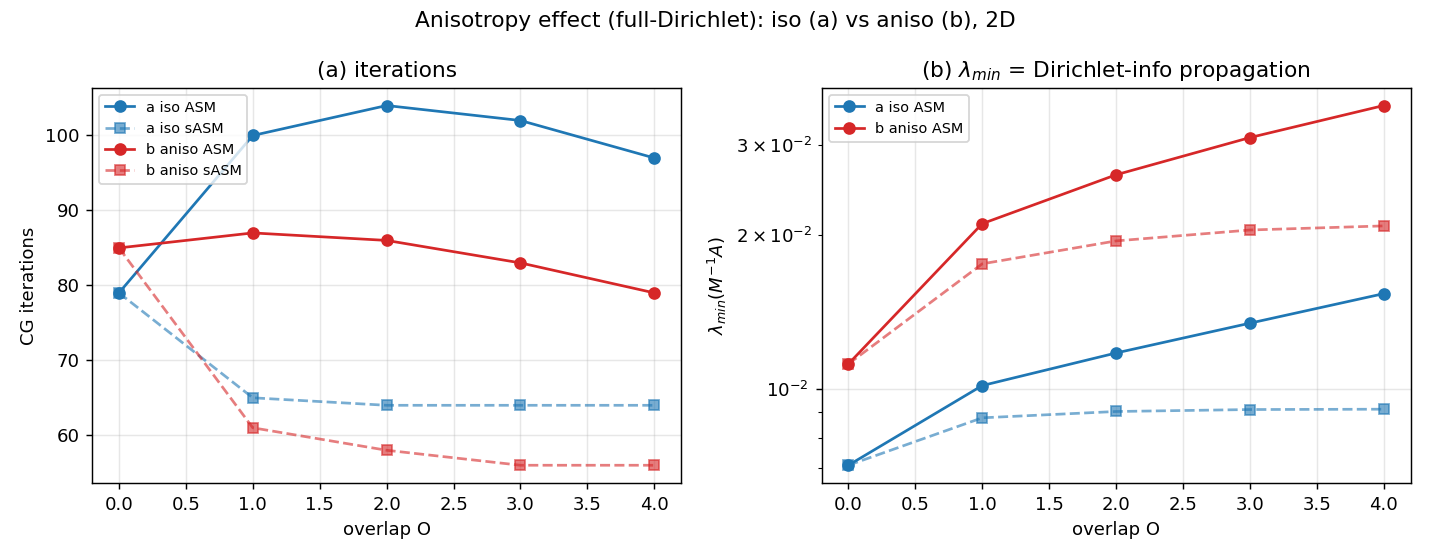
\includegraphics[width=\linewidth,height=0.36\textheight,keepaspectratio]{results/fig_aniso_fullD.png}\\[2pt]
   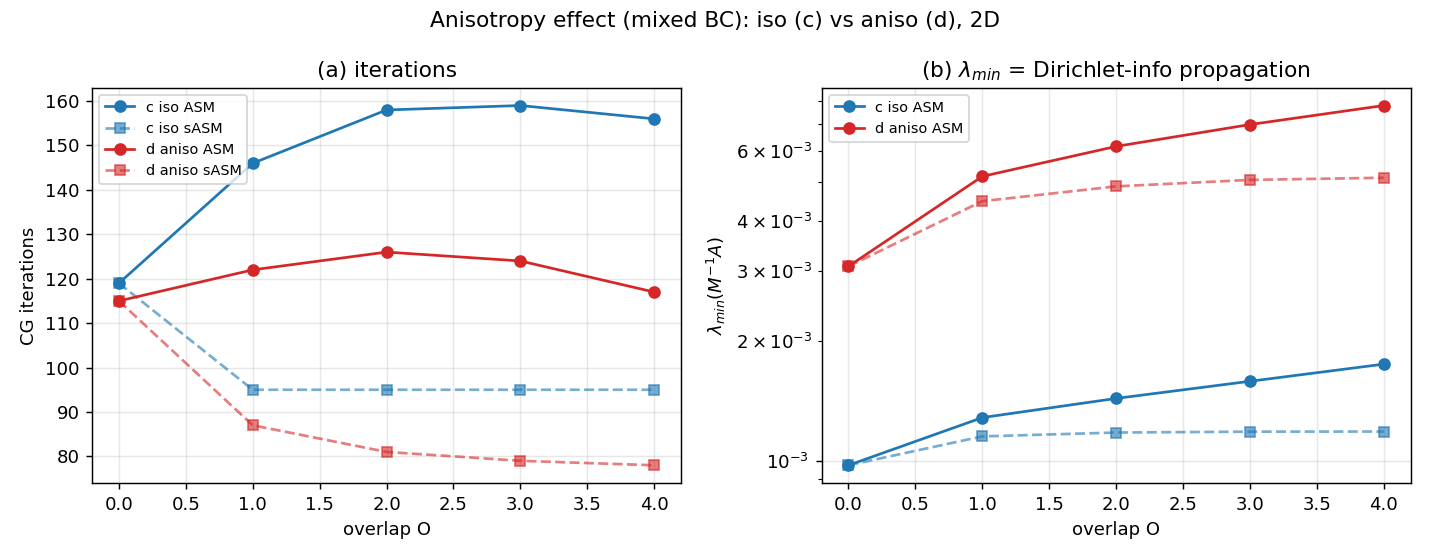
\includegraphics[width=\linewidth,height=0.34\textheight,keepaspectratio]{results/fig_aniso_mixed.png}\\[1pt]
   {\scriptsize\color{muted}\textit{Top: full Dirichlet a (iso) vs b (aniso). Bottom: mixed BC c vs d.}}
  \end{column}
  \begin{column}{0.49\linewidth}\footnotesize
   \begin{itemize}\setlength\itemsep{0.55em}
    \item \cyc effect of anisotropy on iters / $\lambda_{\min}$ under full Dirichlet and mixed BC.
    \item Anisotropy (2D $10\times$, 3D Niederer $7.58$) raises the local ICC amplification $\omega$ and the iteration count.
    \item Geometric over-count $\hat N$ is coefficient-independent (pure geometry); anisotropy does not change it.
    \item \textcolor{sasm}{Worst is case d-3D (anisotropy $\times$ mixed BC): ASM iterations double.}
    \item \textcolor{muted}{sASM removes $\hat N$ and fixes the overlap \emph{trend}, but its geometric weighting is coefficient-blind --- under strong anisotropy / high contrast absolute $\kappa$ stays high, calling for a spectral coarse space (GenEO).}
   \end{itemize}
  \end{column}
  \end{columns}
\end{frame}

% ============================================================= 11 SPECTRUM
\begin{frame}{Spectral distribution (CG Ritz values)}{Interpretability $\cdot$ spectrum}
  \begin{columns}[T]
  \begin{column}{0.66\linewidth}\centering
   \fig[1.0]{fig_spectrum.png}\\[1pt]
   {\scriptsize\color{muted}\textit{Ritz eigenvalues of $M^{-1}A$ at $O{=}2$. Blue = ASM, red = sASM.}}
  \end{column}
  \begin{column}{0.33\linewidth}\footnotesize
   \begin{itemize}\setlength\itemsep{0.6em}
    \item \cyc the preconditioned spectrum.
    \item ASM: a cluster of large eigenvalues to the right ($\hat N$ pushes $\lambda_{\max}$ up).
    \item \textcolor{sasm}{sASM: top end pulled back to $\approx\omega$, spectrum tighter $\Rightarrow$ faster CG.}
    \item \textcolor{muted}{Spectral width $=$ condition number $=$ iteration gap.}
   \end{itemize}
  \end{column}
  \end{columns}
\end{frame}

% ============================================================= 12 TIMING
\begin{frame}{Compute time: sASM slightly dearer per step, faster overall}{Results $\cdot$ time}
  \begin{columns}[T]
  \begin{column}{0.62\linewidth}\centering
   \fig[1.0]{fig_timing_2d.png}\\[1pt]
   {\scriptsize\color{muted}\textit{2D: solve and setup wall time vs overlap. Solid = ASM, dashed = sASM.}}
  \end{column}
  \begin{column}{0.37\linewidth}\footnotesize
   \begin{itemize}\setlength\itemsep{0.5em}
    \item \cyc solve / setup time for ASM and sASM.
    \item sASM adds only two vector scalings ($D^{-1/2}$) per iteration --- negligible overhead.
    \item \textcolor{sasm}{Fewer iterations $\Rightarrow$ sASM total solve time usually shorter.}
    \item \textcolor{muted}{Setup comparable (sASM reuses the same BASIC kernel + one multiplicity pass).}
    \item \textcolor{muted}{Serial timing here (relative comparison); parallel trend on HPC is the same.}
   \end{itemize}
  \end{column}
  \end{columns}
\end{frame}

% ============================================================= 13 CONCLUSIONS
{\setbeamercolor{background canvas}{bg=navy}
\setbeamercolor{normal text}{fg=white}
\begin{frame}[plain]
  \usebeamercolor[fg]{normal text}%
  \vspace{0.4em}{\color{white}\Large\bfseries Conclusions\par}\vspace{0.3em}
  {\color{teal}\rule{\linewidth}{1.5pt}}\vspace{0.6em}
  {\color{white}\footnotesize
  \begin{itemize}\setlength\itemsep{0.55em}
   \item[\textcolor{amber}{\textbf{1}}] \textbf{\textcolor{amber}{sASM beats ASM in 2D/3D across all cases:}} removes the geometric over-count $\hat N$ --- iterations down, $\kappa$ lower, total time shorter, symmetry preserved (CG-safe).
   \item[\textcolor{amber}{\textbf{2}}] \textbf{\textcolor{amber}{1D is the exception:}} ICC(0) exact ($\omega{=}1$), no over-count $\Rightarrow$ no anomaly --- there sASM is slightly worse. sASM is a $d\ge2$ fix.
   \item[\textcolor{amber}{\textbf{3}}] \textbf{\textcolor{amber}{Worst combination:}} 3D + mixed BC + anisotropy (case d-3D), where ASM iterations \emph{double} with overlap.
   \item[\textcolor{amber}{\textbf{4}}] \textbf{\textcolor{amber}{Boundary conditions:}} full Dirichlet lets info enter from all sides $\Rightarrow$ larger $\lambda_{\min}$, milder anomaly; mixed BC the opposite.
   \item[\textcolor{amber}{\textbf{5}}] \textbf{\textcolor{amber}{Mechanism:}} $\lambda_{\max}(\text{ASM})\approx\omega\cdot\hat N$; $\hat N$ = geometric over-count (dimensional amplifier), $\omega$ = inexact-ICC factor (on/off switch).
   \item[\textcolor{amber}{\textbf{6}}] \textbf{\textcolor{amber}{Boundary of the fix:}} sASM's geometric weighting is blind to anisotropy / high contrast --- those need a spectral coarse space (GenEO).
  \end{itemize}}
\end{frame}}

% ============================================================= 14 REPRO
\begin{frame}{Reproduction and tooling}{Appendix}
  \begin{columns}[T]
  \begin{column}{0.57\linewidth}\footnotesize
   \textcolor{teal}{\textbf{Pipeline (PETSc 3.24)}}\\[3pt]
   \texttt{\scriptsize python3 fem\_build.py <a|b|c|d> <dim> <n> <nsub>}\\
   {\scriptsize\color{muted}\ \ unstructured P1 mesh (Delaunay) + assembly +\\ \ \ both partitions $\to$ PETSc binary}\\[3pt]
   \texttt{\scriptsize mpicc schwarz\_fem.c -lpetsc -o schwarz\_fem}\\
   \texttt{\scriptsize bash run\_fem.sh}\ \ {\scriptsize\color{muted}\# all cases $\times$ \{box,METIS\} $\times$ \{ASM,sASM\} $\times O$}\\
   \texttt{\scriptsize python3 parse\_fem.py}\ \ {\scriptsize\color{muted}\# $\to$ CSV + figures}\\[6pt]
   {\scriptsize Measured: iter, $t_{\text{setup}}$, $t_{\text{solve}}$, $\kappa$, Ritz spectrum, $\hat N$, $\omega$.}
  \end{column}
  \begin{column}{0.40\linewidth}\footnotesize
   \textcolor{teal}{\textbf{Notes}}
   \begin{itemize}\setlength\itemsep{0.45em}
     \item Serial + explicit $S^d$/METIS subdomains, independent of rank count.
     \item PETSc 3.24 API --- runs as-is on HPC spack PETSc 3.24 at scale.
     \item High-contrast / anisotropic local ICC uses \texttt{\scriptsize positive\_definite} shift.
     \item Next: add a GenEO spectral coarse space at the case-d boundary.
   \end{itemize}
  \end{column}
  \end{columns}
\end{frame}

\end{document}
